\section{Introduction}


\begin{frame}{Introduction}\framesubtitle{Édition collaborative}

  L'édition collaborative concerne toutes les activités effectuées en
  \textbf{groupe} dans le but de produire un \textbf{document}. L'effort
  collectif permet de bénéficier de multiples points de vues différents.

  \begin{itemize}
  \item[$\rightarrow$] Les documents sont de \textbf{meilleure qualité}.
  \end{itemize}
  
  \vspace{0.25cm}

  \noindent
  \begin{exampleblock}{Le Wikipédia anglais\ldots}
  \begin{minipage}{0.6\textwidth}
    \ldots compte \textbf{5 millions} d'articles, \textbf{40 millions}
      de pages et \textbf{112 mille} utilisateurs actifs.\\Les articles
      possèdent une \textbf{fiabilité} \textbf{comparable} à celle de
      l'Encyclopædia Britannica.
  \end{minipage}\footfullcite{giles2005internet}
  \hfill
  \begin{minipage}{0.3\textwidth}
    \begin{figure}
      \begin{center}
        
\includegraphics[width=0.7\textwidth]{img/wikipedia.png}
      \end{center}
    \end{figure}
  \end{minipage}
  \end{exampleblock}

\end{frame}


\begin{frame}{Introduction}{Éditeur collaboratif Web}
%  \begin{minipage}{0.53\textwidth}
%     Un éditeur collaboratif permet
%     \begin{itemize}
%     \item à \textbf{plusieurs personnes}
%     \item de \textbf{lire} et \textbf{modifier} un document.
%       % \begin{itemize}
%       % \item \textbf{ajout} de caractères
%       % \item \textbf{suppression} de caractères
%       % \end{itemize}
%     \end{itemize}
    
%     Grâce au Web,
%     \begin{itemize}
%     \item n'importe quel outil accédant à l'internet (\textit{e.g. ordinateur,
%         smartphone, tablette}) permet de créer et d'éditer un document aisément.
%     \item Un simple lien permet de le partager facilement avec des amis ou des
%       collègues.
%     \end{itemize}    
% %  \end{minipage}
% %  \begin{minipage}{0.45\textwidth}
%     \begin{figure}    
%       \begin{center}
%         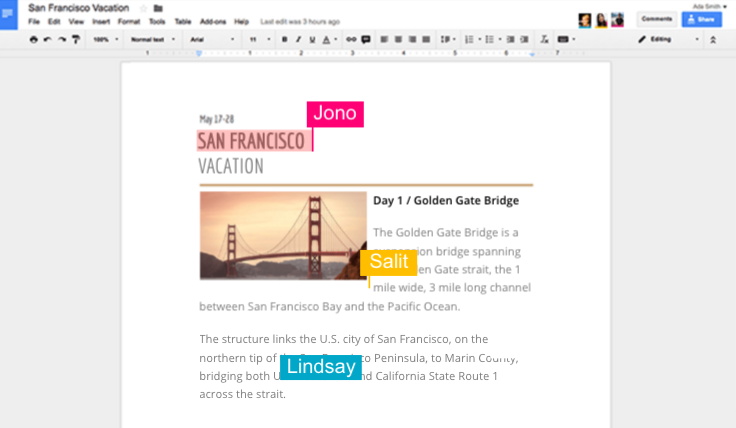
\includegraphics[width=0.65\textwidth]{img/googledocs.png}
% %        \caption{Capture d'écran d'un document Google Docs rédigé par 3 personnes
% %          en simultané. \REF}
%       \end{center}
%     \end{figure}
%  \end{minipage}

  \begin{figure}
    \begin{center}
      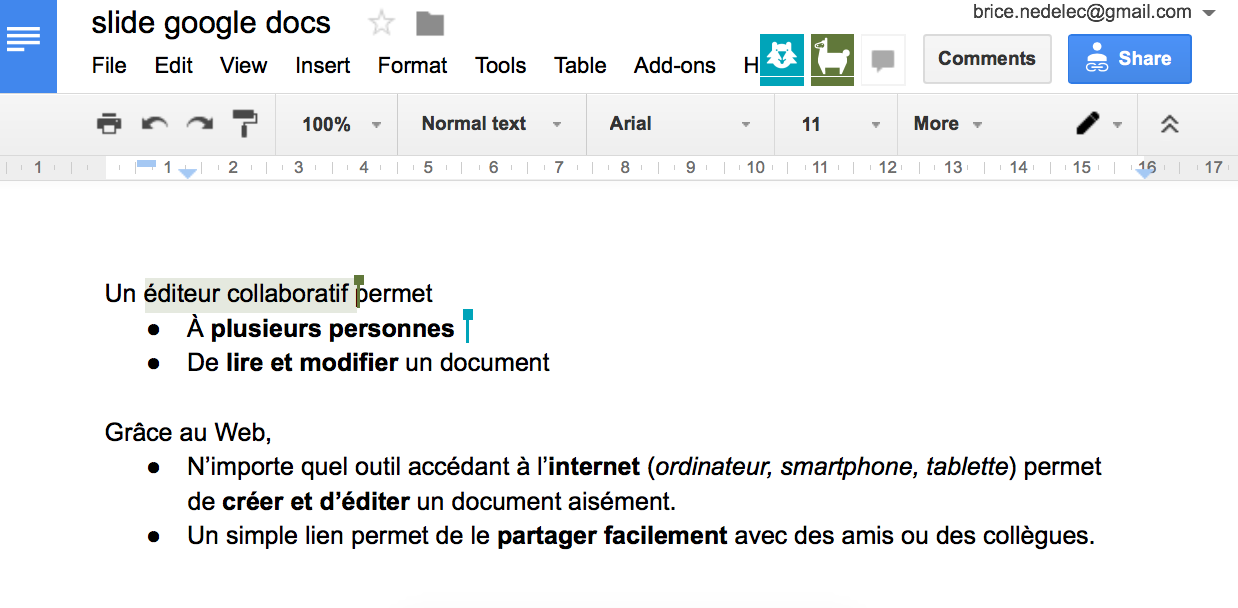
\includegraphics[width=\textwidth]{img/googledocs3.png}\footfullcite{johansen1988groupware}
    \end{center}
  \end{figure}
\end{frame}


\begin{frame}{Introduction}{Problématique}

  % L'organisation du Web est éminemment centralisée : quelques serveurs sont en
  % charge d'un nombre titanesque de clients.
  % \begin{itemize}
  % \item Problèmes de confidentialité, de censure, d'intelligence économique, de
  %   propriété, etc.
  % \item Problèmes de passage à l'échelle et de résilience aux pannes.
  % \end{itemize}
  
  \begin{minipage}{0.69\textwidth}
    Le contexte \textbf{Web} pousse à la \textbf{centralisation :}
    \begin{itemize}
    \item problèmes de \textbf{confidentialité}, \textbf{censure}, etc.
    \uncover<2->{\item problèmes de passage à l'échelle, notamment en \textbf{nombre de
        collaborateurs};}
    \uncover<3->{\item problèmes de \textbf{résilience} aux pannes.}
    \end{itemize}
  \end{minipage}
  \hfill
  \begin{minipage}{0.3\textwidth}
    
\includegraphics[width=0.7\textwidth]{img/www.png}
  \end{minipage}

  \vspace{0.5cm}
  

  \begin{minipage}{0.32\textwidth}
    \begin{center}
      \begin{tikzpicture}
        \node[visible on=<1-3>]
        {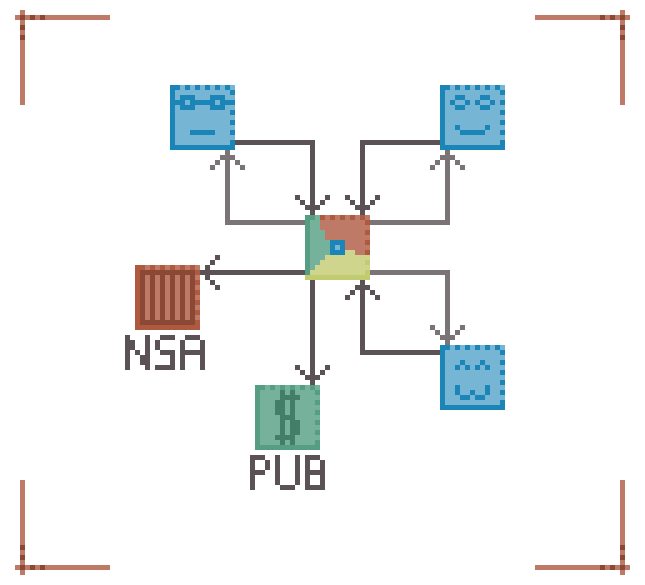
\includegraphics[width=0.95\textwidth]{img/centralizedethicproblems.png}};
      \end{tikzpicture}
    \end{center}
  \end{minipage}
  \begin{minipage}{0.32\textwidth}
    \begin{center}
      \begin{tikzpicture}
        \node[visible on=<2-3>]
        {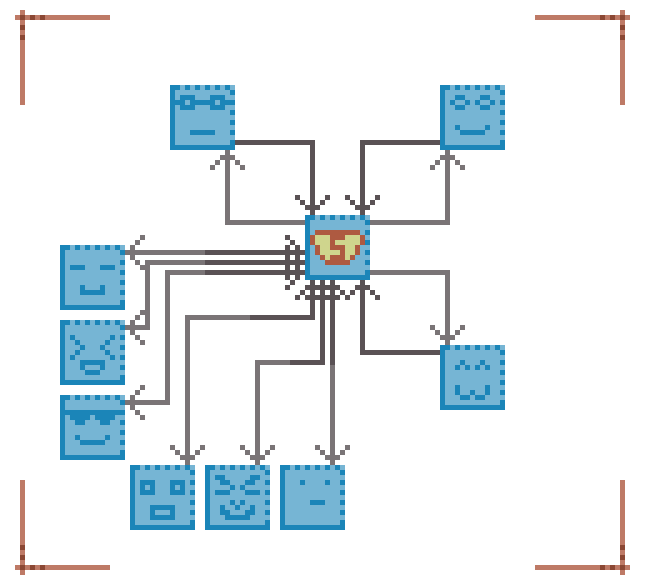
\includegraphics[width=0.95\textwidth]{img/centralizedcpuproblems.png}};
      \end{tikzpicture}
    \end{center}
  \end{minipage}
  \begin{minipage}{0.32\textwidth}
    \begin{center}
      \begin{tikzpicture}
        \node[visible on=<3-3>]
        {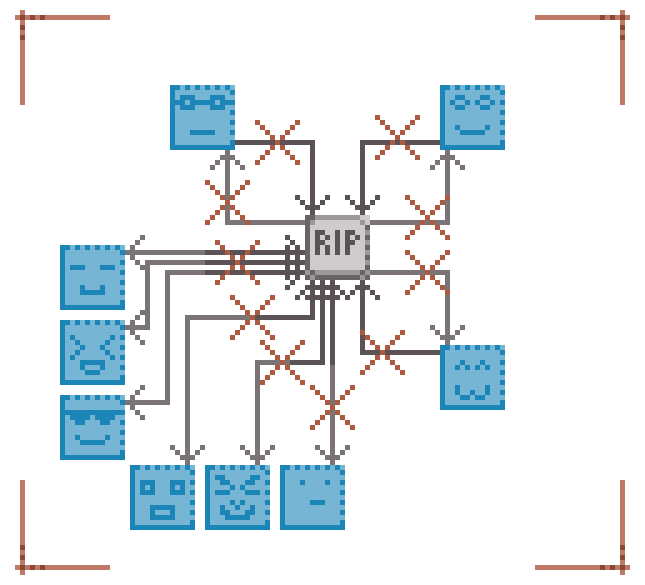
\includegraphics[width=0.95\textwidth]{img/centralizedscalabilityproblems.png}};
      \end{tikzpicture}        
    \end{center}
  \end{minipage}


  \vspace{0.5cm}

  \large\textbf{$\Rightarrow$ L'édition collaborative temps réel est-elle
    possible sur le Web, sans l'intervention d'un tiers et sans limites quant
    aux dimensions du système ?}

\end{frame}


\begin{frame}{Introduction}\framesubtitle{Éditeur collaboratif décentralisé}
  \begin{figure}
    \begin{center}
      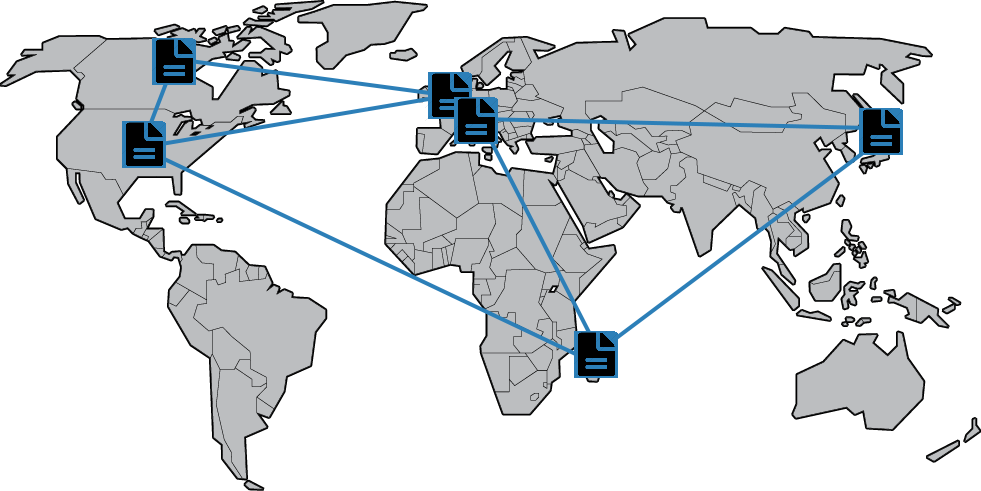
\includegraphics[width=0.8\textwidth]{img/world.png}
    \end{center}
    
    
    \begin{itemize}
    \item Moyen de représenter efficacement un \textbf{document} de manière
      \textbf{cohérente};
    \item Moyen de \textbf{communiquer} efficacement les modifications sur le
      document.
    \end{itemize}

  \end{figure}

  % \begin{itemize}
  % \item Répartition géographique des collaborateurs;
  % \item Édition en temps réel.
  % \end{itemize}
\end{frame}


%%% Local Variables:
%%% mode: latex
%%% TeX-master: "../slides"
%%% End:
